\section{Kinetikus gázelmélet}

\emph{Feltevések; Ideális gáz állapotegyenletének származtatása; Hőmérséklet értelmezése; Ekvipartíció; Szabadsági fokok száma és hőmérsékletfüggése.}

Megismerkedtünk már korábban az ideális gázzal, ami például hélium esetén jó közelítéssel leírja a valódi gáz viselkedését. A valódi gázok leírásával a továbbiakban fogunk még részletesen foglalkozni, azonban először az ideális gázok egyszerű modelljével, a \emph{kinetikus gázelmélettel} ismerkedünk meg. Bernoulli\footnote{Daniel Bernoulli, 1700-1782. Ő ugyanaz a Bernoulli, aki a hidrodinamika Bernoulli-törvényét is kitalálta, azonban egyébként számos híres Bernoulli volt a családban, akik a fizika és a matematika szerteágazó területén tevékenykedtek.} ötlete volt 1738-ban a kinetikus gázelmélet, miszerint tegyük fel, hogy (ennek egy részével már találkoztunk az ideális gázok kapcsán):
\begin{itemize}
    \item a vizsgálandó gázt bezárjuk egy az $x$,$y$,$z$ tengelyek irányával egybeeső kockába, melynek térfogata $V$, az összes részecske száma $N$,
    \item a gázt alkotó atomok vagy molekulák térfogata a gáz által kitöltött térfogathoz képest elhanyagolható, a részecskék pontszerűek, a tömegük legyen $\mu$.
    \item a gázmolekulák egymással ütköznek, azonban más (taszító vagy vonzó) kölcsönhatásban egymással nem állnak,
    \item a gázmolekulák egymással illetve a fallal vett ütközése tökéletesen rugalmas,
    \item mindegyik részecske $v$ sebességgel mozog vagy az $x$,$y$ vagy $z$ tengely irányába, és mindegyik irányba ugyanannyi részecske halad,
    \item a részecskék egyenletesen töltik ki a teret (homogén rendszer, nincs köztük korreláció).
\end{itemize}
Az összeállítás látható \aref{fig:termo_3_1}. ábrán.
\begin{figure}
    \centering
    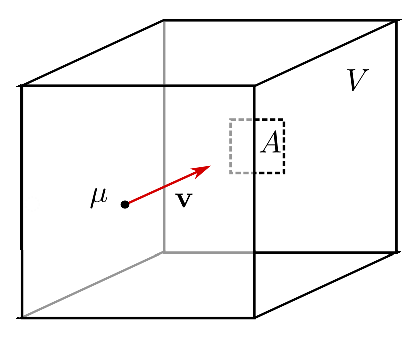
\includegraphics{termo_3/termo_3_1.eps}
    \caption{Ideális gáz kinetikus modellje.}
    \label{fig:termo_3_1}
\end{figure}
Ezen egyszerű feltevések alapján fogjuk meghatározni a rendszer kinetikus energiáját. Bevezetünk néhány jelölést, amit a továbbiakban is használni fogunk\footnote{\,A legtöbb könyv és jegyzet ugyanazt a $p$ betűt használja a nyomásra, impulzusra és a valószínűségre is, az ebből eredő esetleges félreértéseket igyekszünk kikerülni.}. Az impulzust $\mom$, a nagyságát pedig $|\mom|\equiv p$ jelöli. ,,Talpas'' $\prob$ jelöli a valószínűséget, a nyomásra pedig $\pres$ betűvel hivatkozunk. Ismert összefüggések a nyomásra és az erőre, hogy:
\begin{align}
    \pres = \frac FA,\qquad \bm F = \md \mom t.
\end{align}
Vizsgáljunk most a ${+}x$ tengely irányába haladó részecskéket, melyek száma értelemszerűen a feltevéseink alapján $N/6$. Rugalmasan ütköznek a kocka falán, általuk a falra kifejtett nyomás:
\begin{align}
    \pres = \frac{F_x}{A} = \frac{\Delta p_x}{A\cdot \Delta t} = \frac{\frac N6 \mu \cdot \Delta v_x}{A\cdot \Delta t} = \frac{\frac N6 \mu\cdot 2v}{A\cdot \Delta t} = \rec{6A\cdot\Delta t}\frac NV \underbrace{Av\Delta t}_{\equiv V}\cdot 2\mu v = \frac 13 \frac NV \mu v^2.
\end{align}
Ezt kicsit átalakítva kapjuk, hogy:
\begin{align}
    pV = \frac 23 \underbrace{N\frac 12\mu v^2}_{\equiv E_{\tn{kin}}} = \frac 23 E_{\tn{kin}} = nRT,
\end{align}
ahol az utolsó egyenlőségjelnél felhasználtuk az ideális gáz állapotegyenletét. Ebből egyszerű átalakításokkal és a korábban tanult mennyiségekkel adódnak az alábbi relációk:
\begin{align}
    E_{\tn{kin}} = \frac 32 nRT = \frac 32 \frac{N}{N_A} RT = N\frac 12 \mu v^2 \follows \frac 32 \underbrace{\frac{R}{N_A}}_{\equiv k_B} T = \frac 12 \mu v^2,
\end{align}
ahol bevezettük a Boltzmann\footnote{\,Ludwig Boltzmann, 1844-1906.}-állandót, $k_B = R/N_A = 1{,}38\cdot 10^{-23} \tn{J/K}$. Így tehát a gázrészecskék átlagos sebességével, energiájával a hőmérséklet kifejezhető, hiszen egy részecske kinetikus energiája:
\begin{align}\label{eq:ekv_part}
    E_{\tn{1,kin}} = \frac 32 k_B T = \frac 12 \mu v^2 = \frac 12\mu \big(\langle v_x^2 \rangle + \langle v_y^2 \rangle + \langle v_z^2 \rangle\big),
\end{align}
ahol $\langle . \rangle$ egy mennyiség várható értékét\footnote{\,Egy kis valószínűségszámítási ismétlés: diszkrét esetben legyenek egy $x$ mennyiség lehetséges értékei $x_1,x_2,\dots x_N$ rendre $\prob_1,\prob_1,\dots \prob_N$ valószínűséggel. Ekkor az $x$ mennyiség várható értékének nevezzük az $\langle x \rangle = \sum\limits_{i=1}^N \prob_i x_i$ kifejezést ($\sum\limits_{i=1}^N \prob_i = 1$ a mellékfeltétel). Folytonos valószínűségi változónál jelölje $\rho(x)$ a sűrűségfüggvényt ($\int\limits_{-\infty}^\infty \rho(x) \m d x = 1$). Ekkor a várható érték a következő: $\langle x \rangle = \int\limits_{-\infty}^\infty \rho(x)x \m d x$. Hasonlóan értelmezhető például, hogy $\langle x^n \rangle = \int\limits_{-\infty}^\infty \rho(x)x^n \m d x$ tetszőleges $n\in \mathbb N$ számra. Fontos megjegyezni, hogy $\langle x^2\rangle \neq \langle x \rangle ^2$, sőt pont ezeknek a különbsége a szórásnégyzet: $\sigma^2 = \langle (x - \langle x \rangle)^2 \rangle =  \langle x^2\rangle - \langle x \rangle ^2$. Felhasználtuk továbbá a (\ref{eq:ekv_part}). összefüggésben, hogy a határozott integrál integrandusának additivitásából következik, hogy $\langle x_1+x_2 \rangle = \langle x_1 \rangle + \langle x_2 \rangle$.} jelöli. Hélium esetében $300$K-en $\sqrt{\langle v^2 \rangle} \sim 10^4 m/s$. Láthattuk, hogy a rendszer teljes kinetikus energiája $\frac 32 k_BT$. A részecskék a koordináta-rendszer három tengelye ($x$,$y$,$z$) irányába is mozoghatnak, továbbá mivel a sebességnégyzetek várható értéke a három koordinátatengely irányába megegyezik termikus egyensúly esetében, ezért azt mondhatjuk, hogy mindegyik kvandratikus energiatagnak a várható értéke $\frac 12 k_BT$, ezt hívjuk az \emph{ekvipartíció tételének}. Bevezetjük a \emph{szabadsági fokok} számát, amit $f$-fel jelölünk, ez fejezi ki, hogy ,,hány kvadratikus tag van''. Egyatomos ideális gázra $f=3$, kétatomos gázra\footnote{\,Itt már két forgási irányt is meg lehet különböztetni.} $f=5$, többatomos gázra illetve szilárdtestekre\footnote{\,A szilárdtestek atomjai is hőmozgást végeznek, amit modellezhetünk úgy, mint egymáshoz $D$ rugóállandójú rugóval csatolt atomok, ahogy az \aref{fig:termo_3_2}. ábrán is látható. Ez is 3 kvadratikus energiatagot jelenít meg ($\frac 12 D(x^2+y^2+z^2)$), azaz a szabadsági fokok száma: $3 \tn{ mozgási} + 3 \tn{ rugalmas} = 6$.} $f=6$.
\begin{figure}
    \centering
    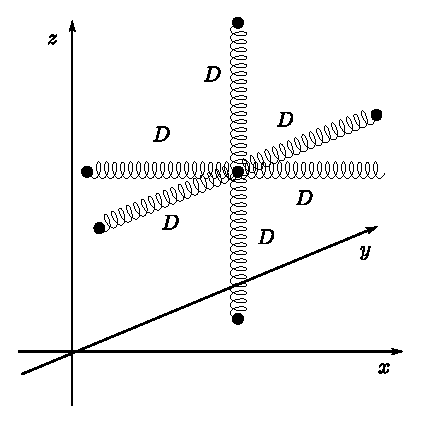
\includegraphics{termo_3/termo_3_2.eps}
    \caption{Szilárdtestek rezgésének modellezése $D$ rugóállandójú rugókkal.}
    \label{fig:termo_3_2}
\end{figure}
A szabadsági fokokkal kifejezve a rendszer kinetikus energiája:
\begin{align}
    E_{\tn{kin}} = \frac f2 Nk_B T.
\end{align}
Általános esetben a dobozba zárt részecskék sebessége nem azonos, hanem az ún. \emph{Maxwell\footnote{\,James Cleck Maxwell, 1831-1879.}--Boltzmann-eloszlást} követik, a részecskék sebességének eloszlása nagyban függ a hőmérséklettől. A Maxwell--Boltzmann-eloszlással később még részletesen fogunk foglalkozni, ezért itt mélyebben nem tárgyaljuk.